\chapter{Vers une Approche de Pronostic Data-Driven}

\chapterintrobox{The goal of this chapter is to introduce the different prognostic approaches with a detailed taxonomy, the various steps of any prognostic approach will be described then the focus will shift towards the data-driven methods.}

\section{Le Pronostic des équipements mécaniques}
Les systèmes complexes surtout dans le domaine de pétrolière fonctionnent sous des conditions très sévères (offshore, désert… ) ce qui peut engendrer l’occurrence des défaillances et leur dégradation. Les pannes et les arrêts non planifiés causent automatiquement des pertes de production, ce qui peut avoir des conséquences économiques énormes. Avec ces contraintes économiques, il faut développer les programmes de maintenance pour minimiser la probabilité des défaillances et le coût. Comme discuté dans l'introduction de ce mémoire, ces programmes doivent être basés sur les principes \acrlong{cbm} et \acrlong{phm}.

Le pronostic et la gestion de la santé (\acrlong{phm}) a deux aspects principaux\cite{Hess2008}:

\begin{enumerate}
    \item \textbf{Pronostic}: diagnostic prédictif, ce qui comprend la détermination de la durée de vie utile restante (durée de bon fonctionnement) d'une composante ou d'un bien.
    \item \textbf{Gestion de la santé}: la capabilité de prendre des décisions concernant les actions de maintenance en basant sur les informations du diagnostic/pronostic, les ressources disponibles et la demande opérationnelle.
\end{enumerate}

\section{Estimation de durée de vie utile restante}
L'objectif principal du pronostic c'est l'estimation de la durée de vie utile restante (\acrlong{rul}) du système.
\acrshort{rul} est défini selon l'équation \ref{eq:rul}:

\begin{equation}
    RUL = t_f-t_c
    \label{eq:rul}
\end{equation}

Où $t_f$ est le temps prédit pour l’occurrence de la défaillance et $t_c$ est le temps actuel (le temps quand la prédiction est faite).
%TODO: discussion of abstraction levels for RUL estimation

\section{Approches Physiques, Data-Driven et Hybrides}
Toute approche pronostique peut être basée sur des modèles physiques, modèles data-driven ou une combinaison hybride des deux (Figure \ref{fig:prognostic-approaches-venn}).

\begin{figure}[h]
    \centering
	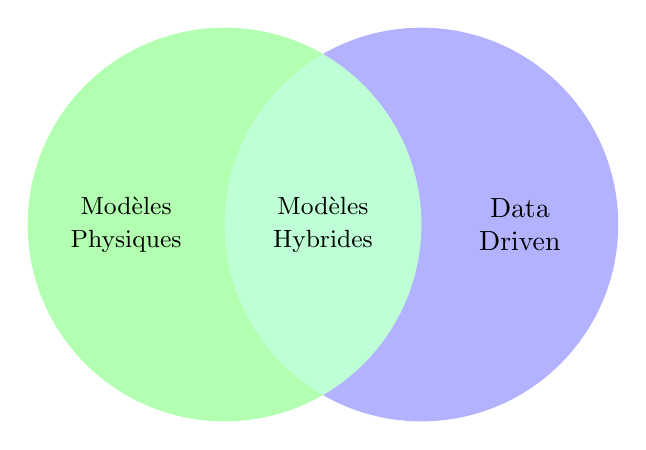
\begin{tikzpicture}
\begin{scope}
[blend group = soft light]
\fill [green!30!white] (0,0) circle (2.5);
\fill [blue!30!white] (2.5,0) circle (2.5);
\end{scope}

\node[text width=2cm, align=center] at (-1.25,0) {\small Modèles Physiques};
\node[text width=1.5cm, align=center] at (3.75,0) { Data Driven};
\node[text width=1.6cm, align=center] at (1.25,0) {\small Modèles Hybrides};
\end{tikzpicture}

    \caption{Classification des approches de pronostic}
    \label{fig:prognostic-approaches-venn}
\end{figure}

Ces trois catégories constituent une classification générale fondée sur l'approche suivie, chacune d'entre elles pouvant être subdivisée en sous-catégories. Une taxonomie détaillée est présentée à la figure \ref{fig:prognostic-approaches-tree}.
\begin{figure}[H]
	\resizebox{\textwidth}{!}{
\begin{tikzpicture}
	[all/.style={draw, minimum height=2em, fill=white, font=\small}]

	\fill [gray!30!white] (-1.41,-6.3) rectangle (1.41,-9.7) ;
	
	\draw(0,0) node[all] (progApp)                       	{Les Approches du Pronostic};
	\draw node[all, below = 1.6em of progApp] (dataDriv)		{Data-Driven};
	\draw node[all, left = 7em of dataDriv] (physBas)      	{Modèles Physiques};
	\draw node[all, right = 7em of dataDriv] (hybridApp)				{Modèles Hybrides};

	\draw node[all,text width=2cm,align=center,minimum height=3em, below = 1.6em of physBas] (appSpec)		{Application Specific};
	
	\begin{scope}[node distance=1.6em and -3.5em]
		\draw node[all,text width=2cm,align=center,minimum height=3em, below right = of hybridApp] (serApp)		{Approches en Série};
		\draw node[all,text width=2cm,align=center,minimum height=3em, below left = of hybridApp] (parApp)		{Approches Parallèles};
	\end{scope}
	
	\begin{scope}[node distance=1.6em and -2.5em]
		\draw node[all,text width=2cm,align=center,minimum height=3em, below right = of dataDriv] (statMod)		{Modèles Statistiques};
		\draw node[all,text width=2cm,minimum height=3em, align=center, below left = of dataDriv] (ML)		{Machine Learning};
	\end{scope}

	\begin{scope}[node distance=1.6em and 0em]
		\draw node[xshift=1em,all,text width=2.9cm,align=center,minimum height=3em, below left = of ML] (connect) {Méthodes Connectionnistes};
		\draw node[all,text width=2.9cm,align=center,minimum height=3em, below = of connect] (instance) {Apprentissage Contextuel};
		\draw node[ all,text width=2.9cm,align=center,minimum height=3em, below = of instance] (comb)		{Méthodes Combinées};
	\end{scope}

	\begin{scope}[node distance=1.6em and 0em]
		\draw node[xshift=-1em,all,text width=2.9cm,align=center,minimum height=3em, below right = of statMod] (reg)		{Méthodes de Regression};
		\draw node[all,text width=2.9cm,align=center,minimum height=3em, below = of reg] (arma)		{ARMA \& variantes};
		\draw node[all,text width=2.9cm,align=center,minimum height=3em, below = of arma] (propor)		{Modèle à Risque Proportionnel};
	\end{scope}

	\begin{scope}[node distance=1.6em and 0em]
	\path let \p1 = (connect) in node[all,text width=2.3cm,align=center,minimum height=3em] (bayes)	at (0,\y1)	{Méthodes Bayésiennes};
	\draw node[all,text width=2.3cm,align=center,minimum height=3em, below  = of bayes] (hmm)		{Modèles de Markov};
	\draw node[all,text width=2.3cm,align=center,minimum height=3em, below  = of hmm] (sotch)		{Filtrage Stochastique};
	\end{scope}

	\draw[->, >=angle 60] (progApp.south)   -- ++(0,0) -- ++(0,-0.8em) -| (physBas.north);
	\draw[->, >=angle 60] (progApp.south)   -- ++(0,0) -- ++(0,-0.8em) -| (hybridApp.north);
	\draw[->, >=angle 60] (progApp.south)   --  (dataDriv.north);
	
	\draw[->, >=angle 60] (physBas.south)   --  (appSpec.north);
	
	\draw[->, >=angle 60] (hybridApp.south)   -- ++(0,0) -- ++(0,-0.8em) -| (parApp.north);
	\draw[->, >=angle 60] (hybridApp.south)   -- ++(0,0) -- ++(0,-0.8em) -| (serApp.north);
	
	\draw[->, >=angle 60] (dataDriv.south)   -- ++(0,0) -- ++(0,-0.8em) -| (statMod.north);
	\draw[->, >=angle 60] (dataDriv.south)   -- ++(0,0) -- ++(0,-0.8em) -| (ML.north);
	
	\draw[->, >=angle 60] ([xshift=-1em]ML.south)   |- (connect.east);
	\draw[->, >=angle 60] ([xshift=-1em]ML.south)   |- (instance.east);
	\draw[->, >=angle 60] ([xshift=-1em]ML.south)   |- (comb.east);
	
	\draw[->, >=angle 60] ([xshift=1em]statMod.south)   |- (reg.west);
	\draw[->, >=angle 60] ([xshift=1em]statMod.south)   |- (arma.west);
	\draw[->, >=angle 60] ([xshift=1em]statMod.south)   |- (propor.west);

	\draw[->, >=angle 60] (ML.south)   -- ++(0,0) -- ++(0,-0.8em) -| (bayes.north);
	\draw[-] (statMod.south)   -- ++(0,0) -- ++(0,-0.8em) -| (bayes.north);
	\draw[->, >=angle 60] (bayes.south)   -- (hmm.north);
\end{tikzpicture}
}
    \caption{Taxonomie des approches de pronostic \cite{Javed2017}}
    \label{fig:prognostic-approaches-tree}
\end{figure}

\subsection{Modèles Physiques}
Les modèles physiques évaluent la santé du système en utilisant une formulation mathématique explicite (boîtes blanches) développée sur la base d'une compréhension scientifique et technique de son comportement. Cependant, le principal avantage de ces modèles physiques consiste à utiliser des modèles de dégradation pour prédire le comportement à long terme \cite{Cubillo2016}. Les approches physiques sont capables de fournir une estimation précise de \acrshort{rul} si le modèle physique est développé avec une compréhension complète des mécanismes de défaillance et une estimation efficace des paramètres du modèle. Cependant, pour certains systèmes mécaniques complexes, il est difficile de comprendre la physique des dommages, ce qui limite l'application de ces approches \cite{Lei2018}.

\subsection{Modèles Data-Driven}
Les modèles \acrshort{dd} s'appuient sur des données collectées précédemment (données de surveillance, données sur les paramètres opérationnels, ... ) pour établir un modèle capable d'évaluer la santé du système et de prévoir son comportement et sa dégradation. Contrairement aux modèles physiques, et comme leur nom l'indique, les modèles \acrshort{dd} ne s'appuient pas sur les connaissances humaines mais principalement sur les données historiques collectées pour modéliser le processus de dégradation. Habituellement, ils sont considérés comme des boîtes noires.

\subsubsection{Modèles Statistiques}
L'approche statistique, pour l'estimation des \acrshort{rul}, repose sur la construction et l'ajustement d'un modèle probabiliste en utilisant les données historiques sans dépendre d'aucun principe physique ou technique \cite{Si2011}. 
Si et al. \cite{Si2011} ont présenté une revue des approches statistiques. Selon cette revue, de nombreux modèles entrent dans cette catégorie tels que les modèles de régression (e.g. la régression linéaire), la moyenne mobile autorégressive et ses variantes, les techniques de filtrage stochastique (e.g. filtre de Kalman, filtre particulaire, ...).

\subsubsection{Machine Learning}
L'apprentissage automatique est un domaine de l'intelligence artificielle qui a explosé ces dernières années et a fait des percées dans de nombreux domaines tels que Computer Vision et Natural Language Processing. Les modèles d'apprentissage automatique sont des modèles boîte noire qui permettent de découvrir des mappages même très complexes d'une entrée à une sortie. De nombreux types d'algorithmes entrent dans cette catégorie comme les méthodes connectionnistes (e.g. les réseaux neuronaux artificiels), l'apprentissage contextuel (e.g. les machine à vecteurs de support). Différentes approches peuvent être combinées ensemble pour créer des modèles mixte qui peuvent être plus performants qu'un modèle unique.

\subsection{Modèles Hybrides}
Les modèles hybrides sont une combinaison d'un modèle physique et d'un modèle \acrlong{dd}. Il existe deux types de modèles hybrides selon la façon dont les deux types des modèles sont combinés. Le modèle \acrlong{dd} peut être intégré dans un modèle physique en configuration série (Figure \ref{fig:hybrid-approach-series}) où il est utilisé pour ajuster les paramètres du modèle physique qui utilisé alors pour faire des prédictions.

\begin{figure}[H]
    \centering
    \begin{tikzpicture}
 	\node[draw, rectangle] (ph) {Physics based approach};
 	\node[draw, rectangle, below = 3em of ph] (dd) {Data-driven approach};
 	
 	\draw[->, >=angle 60] (dd.north) -- node[right] {\scriptsize  Parameter tuning} (ph.south);
 	\draw[->, >=angle 60] (ph.east) -- node[above] {\scriptsize Prediction} ([xshift=4.5em]ph.east);
 	\draw[->, >=angle 60] (-4.5,0) -- node[above] {\scriptsize Input} (ph.west);
	\draw[->, >=angle 60] (-3,0) |-  (dd.west);
\end{tikzpicture}
    \caption{Configuration hybride en série (Figure adaptée de la référence \cite{Mangili2013})}
    \label{fig:hybrid-approach-series}
\end{figure}

Les deux types de modèles peuvent être combinés dans une configuration parallèle (Figure \ref{fig:hybrid-approach-parallel}) où les deux modèles font des prédictions séparées qui peuvent être combinées pour obtenir l'estimation finale.
\begin{figure}[H]
    \centering
    \begin{tikzpicture}
    \node[draw, rectangle] (ph) {Physics based approach};
    \node[draw, circle, below = 1em of ph] (u) {U};
    \node[draw, rectangle, below = 1em of u] (dd) {Data-driven approach};

    \draw[->, >=angle 60] (u.east)      --      node[above] {\scriptsize Prediction} ([xshift=4.5em]u.east);
    \draw[->, >=angle 60] (ph.south)    --      (u.north);
    \draw[->, >=angle 60] (dd.north)    --      (u.south);
    \draw[->, >=angle 60] (-4.5,0)      --      node[above] {\scriptsize Input} (ph.west);
    \draw[->, >=angle 60] (-3,0)        |-      (dd.west);
    %the following lign is just to make the figure center precisely and align with the previous one
    \draw[->, draw=none] (ph.east) -- ([xshift=4.5em]ph.east);
\end{tikzpicture}
    \caption{Configuration hybride parallèle (Figure adaptée de la référence \cite{Mangili2013})}
    \label{fig:hybrid-approach-parallel}
\end{figure}

\section{Pourquoi une approche Data-Driven?}
Comme mentionné précédemment, comprendre le processus de dégradation pour les systèmes très complexes est extrêmement difficile, c'est pourquoi le développement des modèles physiques est très problématique pour ces systèmes.

Les 20 dernières années ont vu de grands progrès dans le développement de nouvelles techniques de détection, de méthodes de pronostic/diagnostic et dans l’application des méthodes d’analyse informatisées. 

Il est intéressant de noter que, lors de l’atelier de 2002 sur la maintenance conditionnelle organisé par Advanced Technology Program du National Institute of Standards and Technology (NIST) des États-Unis, les obstaces suivants à l’application généralisée des mesures de confiance ont été identifiés :
\begin{itemize}%[label=$\bullet$]
    \item L’impossibilité de prédire avec exactitude et fiabilité la durée de vie utile restante d'une machine.
    \item L’incapacité de surveiller continuellement une machine.
    \item L’incapacité des systèmes de maintenance à apprendre et à identifier les défaillances imminentes et à recommander les mesures à prendre.
\end{itemize} 

Ces obstacles peuvent être redéfinis comme des déficiences au niveau des pronostics, de la détection et du raisonnement. Ces limitations et d'autres encore de la mise en œuvre actuelle des techniques de maintenance conditionnelle ont, bien entendu, été reconnues par d'autres et ont conduit à l'élaboration de programmes (e.g. dans le domaine militaire) visant à les surmonter \cite{Hess2008}.

Aujourd'hui, les capteurs dans l'industrie sont devenus peu coûteux et omniprésents, la puissance de calcul a augmenté exponentiellement ce qui a permis de dévlopper des algorithmes et outils informatiques plus avancés : la révolution de l'intelligence artificielle et l'apprentissage automatique. L’industrie génère d’énormes quantités de données dans de nombreux domaines dont la majorité est inexploitée, l’exploitation de ces données en utilisant les dernières avancées technologiques peut augmenter les profits, réduire les coûts de manière drastique et s’avérer être un énorme avantage économique.

\section{Conclusion}
%TODO: finish this shit too